\documentclass[12pt]{article}
\usepackage[utf8]{inputenc}
\usepackage{upquote}
\usepackage[margin=1in]{geometry} 
\usepackage{amsmath,amsthm,amssymb}
\usepackage{graphicx}
\usepackage{listings}
\newenvironment{statement}[2][Statement]{\begin{trivlist}
\item[\hskip \labelsep {\bfseries #1}\hskip \labelsep {\bfseries #2.}]}{\end{trivlist}}
\usepackage{xcolor}




\title{Assignment 6}


\author{Author \\
  Wanjing Hu / fng685@alumni.ku.dk  \\
  Zhigao Yan / sxd343@alumni.ku.dk  \\
  Wenshuo Dong / gnj461@alumni.ku.dk  \\
  Jiayi Zhang / xrw579@alumni.ku.dk \\
} 
 

\begin{document}
\maketitle

\section{Question1 $P_1$}
%zhigao
\begin{figure}[h]
    \centering
    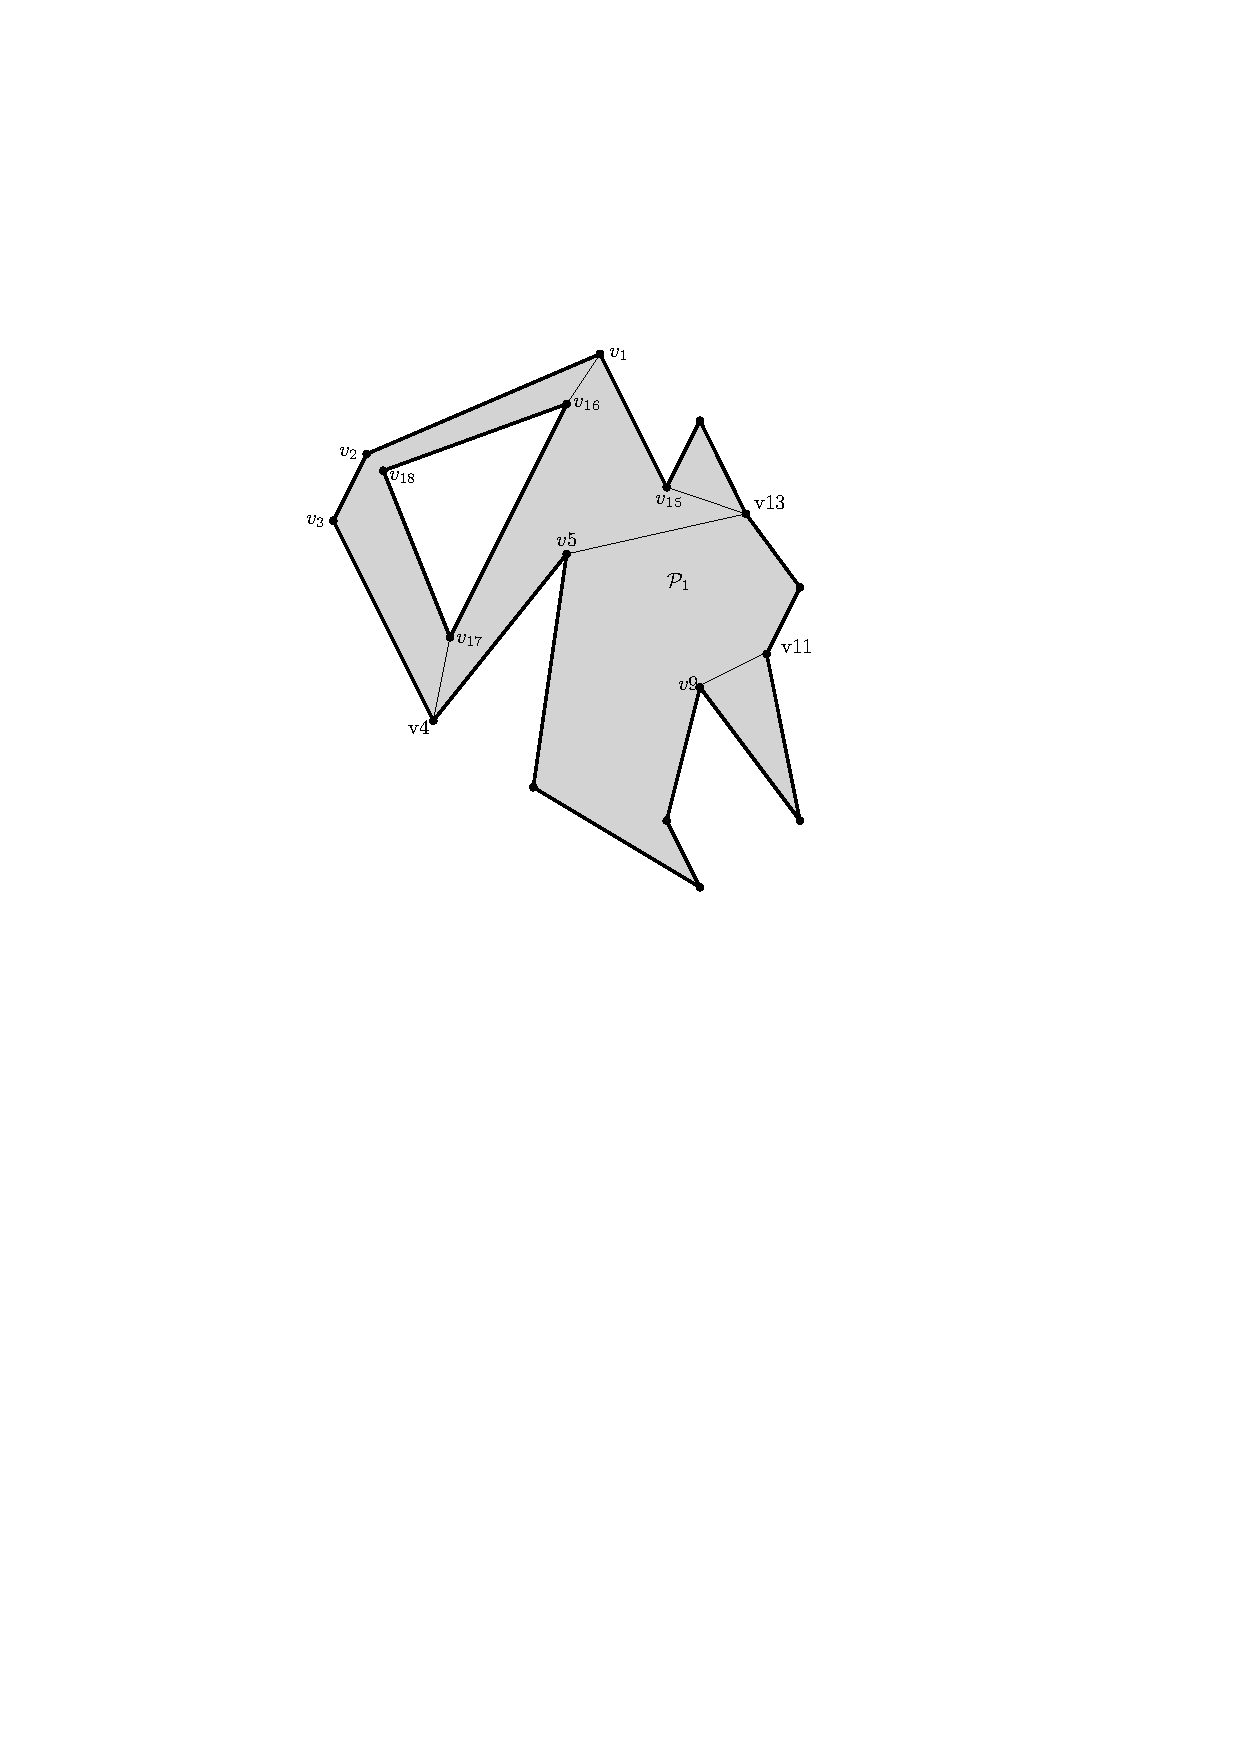
\includegraphics[width=0.5\linewidth]{triangulationExercise (2)-1.pdf}
    \caption{Question 1}
    \label{fig:enter-label}
\end{figure}
I use the method from the Computational Geometry book that handles everything in one pass.
The order of the diagonal that I created:

\[v_{16} \rightarrow v_1\]
\[v_{13} \rightarrow v_15\]
\[v_{5} \rightarrow v_{13}\]
\[v_{9} \rightarrow v_{11}\]
\[v_{4} \rightarrow v_{17}\]



\section{Question1 $P_2$}
%wenshuo

\section{Exercises 3.4}
%jiayi

\section{Exercises 3.7}
%wanjing

\end{document}
